\documentclass[12pt]{beamer}
%\usepackage{mystyle}

% Since <T>LAPACK does not properly render in LaTeX without putting < in math mode,
%   we define the following command to make referencing it more convenient
\newcommand{\tla}{$<$T$>$LAPACK}

\author{Johnathan Rhyne}
\title{Developing with \tla}

\begin{document}
    \begin{frame}
        \maketitle
    \end{frame}
    \begin{frame}
        \tableofcontents
    \end{frame}
    \section{Developing for \tla}
    \begin{frame}
        \frametitle{Developing for \tla}
        % This will serve as a reminder slide for the users mostly to draw attention to the templating behavior
        As was said before, the codebase for \tla is written in header files. This allows us to 
        take advantage of templates!
    \end{frame}
    \section{My project within \tla}
    \begin{frame}
        \frametitle{My project within \tla}
        Discuss how I wrote the code for 
        I worked on some software that was for a fork of \tla. The code can be found here: 
        \url{https://github.com/jprhyne/tlapack/tree/hqr}.
    \end{frame}
    \begin{frame}
        \frametitle{My project within \tla}
        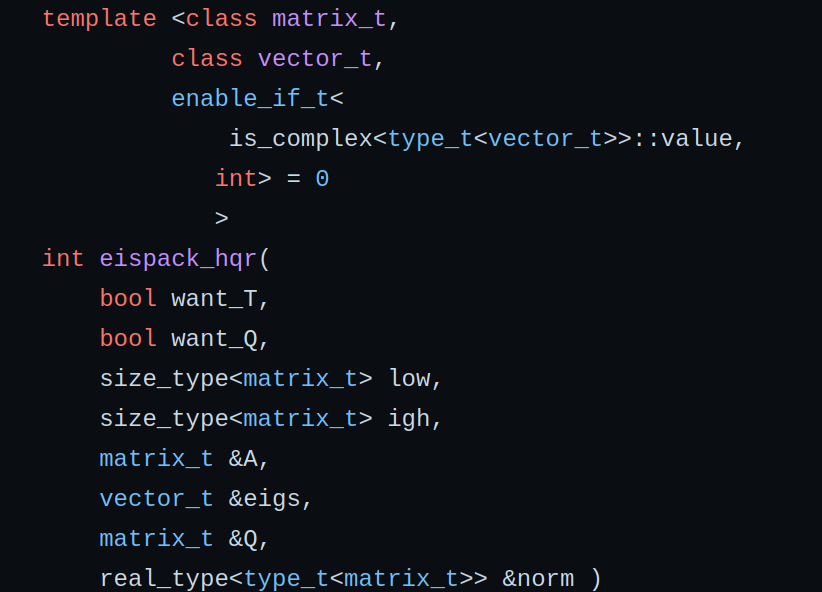
\includegraphics[width=\textwidth]{images/eispackHqr.png}
        % This slide mainly serves as a talking point. Depending on what is talked about previously I may 
        % make this brief and treat it as a showcase of the interface. Or go into some more detail
        % centering around the top part (unsure what will be covered prior to me talking)
    \end{frame}
    \begin{frame}
        \frametitle{My workflow}
        \begin{enumerate}
            \item Write in a language I am comfortable with (C)
            \item Segment the code (create more functions!)
            \item Transcribe a function at a time along with white-box testing
            \item Transcribe the main driver
        \end{enumerate}
    \end{frame}
    \section{Examples of calling code}
    \begin{frame}
        \frametitle{Examples of calling code}
        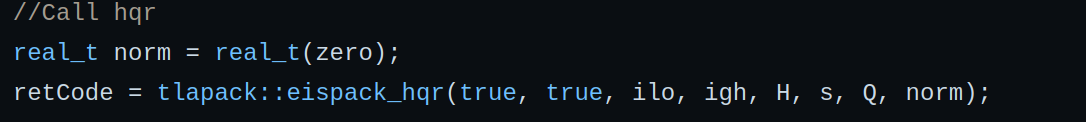
\includegraphics[width=\textwidth]{images/callingHqr.png}
        Looking at the testing files, we don't need to do anything special in order to call our templated
        functions. In fact, it is very similar to how you would use an interface like CBLAS or LAPACKE.

        It's possible to omit the namespace dereference in the function calls, but the way to do so is 
        not good practice for C++
    \end{frame}
    \section{Timing of my project}
    \begin{frame}
        \frametitle{Timing of my project}
        Present some timing (performance) of things in email thread to show how we might use this as well as 
        some motivation about why we care

%       Note: Having trouble compiling my current repo as the newest version of Catch2 doesn't play nice with
%       the old version of the repository. Currently investigating ways to work around this problem (trying an old
%       version of gcc as some other things I've found online have this as a solution to this problem
%       Another option is to create a new branch based on current main and then manually copy the files over one 
%       at a time. The former is preferred for building purposes

% Goal is to have 4-7 slides detailing numerical experiments
    \end{frame}
    \section{Differing precisions}
    \begin{frame}
        \frametitle{Differing precisions}
        Some users already use the ease of the templating to use non-standard precisions. For example, this
        user was testing 8-bit floating point arithmetic, and only had to change how data was declared.
        \url{https://github.com/SudhanvaKulkarni123/tlapack}
        % Will try to get some more stuff for this section
    \end{frame}
\end{document}
